\documentclass[]{article}
\usepackage[T1]{fontenc}
\usepackage{lmodern}
\usepackage{amssymb,amsmath}
\usepackage{ifxetex,ifluatex}
\usepackage{fixltx2e} % provides \textsubscript
% use upquote if available, for straight quotes in verbatim environments
\IfFileExists{upquote.sty}{\usepackage{upquote}}{}
\ifnum 0\ifxetex 1\fi\ifluatex 1\fi=0 % if pdftex
  \usepackage[utf8]{inputenc}
\else % if luatex or xelatex
  \ifxetex
    \usepackage{mathspec}
    \usepackage{xltxtra,xunicode}
  \else
    \usepackage{fontspec}
  \fi
  \defaultfontfeatures{Mapping=tex-text,Scale=MatchLowercase}
  \newcommand{\euro}{€}
\fi
% use microtype if available
\IfFileExists{microtype.sty}{\usepackage{microtype}}{}
\usepackage[margin=1in]{geometry}
\usepackage{color}
\usepackage{fancyvrb}
\newcommand{\VerbBar}{|}
\newcommand{\VERB}{\Verb[commandchars=\\\{\}]}
\DefineVerbatimEnvironment{Highlighting}{Verbatim}{commandchars=\\\{\}}
% Add ',fontsize=\small' for more characters per line
\usepackage{framed}
\definecolor{shadecolor}{RGB}{248,248,248}
\newenvironment{Shaded}{\begin{snugshade}}{\end{snugshade}}
\newcommand{\KeywordTok}[1]{\textcolor[rgb]{0.13,0.29,0.53}{\textbf{{#1}}}}
\newcommand{\DataTypeTok}[1]{\textcolor[rgb]{0.13,0.29,0.53}{{#1}}}
\newcommand{\DecValTok}[1]{\textcolor[rgb]{0.00,0.00,0.81}{{#1}}}
\newcommand{\BaseNTok}[1]{\textcolor[rgb]{0.00,0.00,0.81}{{#1}}}
\newcommand{\FloatTok}[1]{\textcolor[rgb]{0.00,0.00,0.81}{{#1}}}
\newcommand{\CharTok}[1]{\textcolor[rgb]{0.31,0.60,0.02}{{#1}}}
\newcommand{\StringTok}[1]{\textcolor[rgb]{0.31,0.60,0.02}{{#1}}}
\newcommand{\CommentTok}[1]{\textcolor[rgb]{0.56,0.35,0.01}{\textit{{#1}}}}
\newcommand{\OtherTok}[1]{\textcolor[rgb]{0.56,0.35,0.01}{{#1}}}
\newcommand{\AlertTok}[1]{\textcolor[rgb]{0.94,0.16,0.16}{{#1}}}
\newcommand{\FunctionTok}[1]{\textcolor[rgb]{0.00,0.00,0.00}{{#1}}}
\newcommand{\RegionMarkerTok}[1]{{#1}}
\newcommand{\ErrorTok}[1]{\textbf{{#1}}}
\newcommand{\NormalTok}[1]{{#1}}
\usepackage{graphicx}
% Redefine \includegraphics so that, unless explicit options are
% given, the image width will not exceed the width of the page.
% Images get their normal width if they fit onto the page, but
% are scaled down if they would overflow the margins.
\makeatletter
\def\ScaleIfNeeded{%
  \ifdim\Gin@nat@width>\linewidth
    \linewidth
  \else
    \Gin@nat@width
  \fi
}
\makeatother
\let\Oldincludegraphics\includegraphics
{%
 \catcode`\@=11\relax%
 \gdef\includegraphics{\@ifnextchar[{\Oldincludegraphics}{\Oldincludegraphics[width=\ScaleIfNeeded]}}%
}%
\ifxetex
  \usepackage[setpagesize=false, % page size defined by xetex
              unicode=false, % unicode breaks when used with xetex
              xetex]{hyperref}
\else
  \usepackage[unicode=true]{hyperref}
\fi
\hypersetup{breaklinks=true,
            bookmarks=true,
            pdfauthor={},
            pdftitle={},
            colorlinks=true,
            citecolor=blue,
            urlcolor=blue,
            linkcolor=magenta,
            pdfborder={0 0 0}}
\urlstyle{same}  % don't use monospace font for urls
\setlength{\parindent}{0pt}
\setlength{\parskip}{6pt plus 2pt minus 1pt}
\setlength{\emergencystretch}{3em}  % prevent overfull lines
\setcounter{secnumdepth}{5}

\title{STAT 133 Final Report }
\author{Student: Xi Chen, SID: 22824137}
\date{}

\begin{document}

\normalsize


% {
% \hypersetup{linkcolor=black}
% \setcounter{tocdepth}{2}
% \tableofcontents
% }

\maketitle


\section{Preliminary Data Analysis}\label{preliminary-data-analysis}

First we analyze the if some questions are omitted more than others:

\begin{Shaded}
\begin{Highlighting}[]
\NormalTok{filtered.data =}\StringTok{ }\KeywordTok{read.table}\NormalTok{(}\StringTok{"ling-data-clean.data"}\NormalTok{, }\DataTypeTok{header=}\NormalTok{T)}
\NormalTok{vars =}\StringTok{ }\KeywordTok{grep}\NormalTok{(}\StringTok{"Q"}\NormalTok{, }\KeywordTok{colnames}\NormalTok{(filtered.data), }\DataTypeTok{value=}\NormalTok{T)}
\NormalTok{omitted.count =}\StringTok{ }\KeywordTok{apply}\NormalTok{(filtered.data[, vars] ==}\StringTok{ }\DecValTok{0}\NormalTok{, sum, }\DataTypeTok{MARGIN=}\KeywordTok{c}\NormalTok{(}\DecValTok{2}\NormalTok{)) }\CommentTok{# filtered.data is raw data with specified obs removed}
\KeywordTok{barplot}\NormalTok{(omitted.count)}
\end{Highlighting}
\end{Shaded}

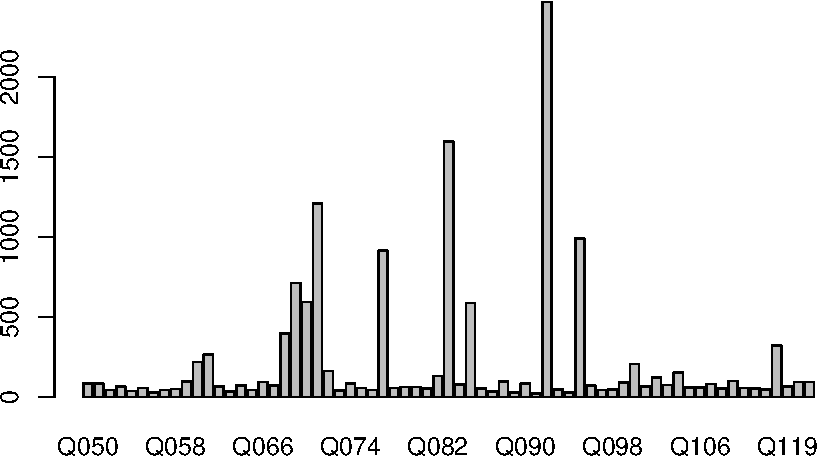
\includegraphics{./writeup_files/figure-latex/unnamed-chunk-1.pdf}

It's evident from the bar plot that certain questions are omitted
significantly more than others. Next we will analyze what are the
outliers and if the exclusion is related to geography:

\begin{Shaded}
\begin{Highlighting}[]
\NormalTok{outliers =}\StringTok{ }\KeywordTok{names}\NormalTok{(omitted.count[omitted.count >}\StringTok{ }\KeywordTok{quantile}\NormalTok{(omitted.count, }\DataTypeTok{probs=}\KeywordTok{c}\NormalTok{(}\FloatTok{0.95}\NormalTok{))])}
\KeywordTok{print}\NormalTok{(outliers)}
\end{Highlighting}
\end{Shaded}

\begin{verbatim}
## [1] "Q071" "Q083" "Q092" "Q095"
\end{verbatim}

\begin{Shaded}
\begin{Highlighting}[]
\NormalTok{omitters.ind =}\StringTok{ }\NormalTok{filtered.data[, outliers] ==}\StringTok{ }\DecValTok{0}
\NormalTok{omitters =}\StringTok{ }\NormalTok{filtered.data[omitters.ind, ]}
\KeywordTok{plot}\NormalTok{(filtered.data[-omitters.ind, }\StringTok{"lat"}\NormalTok{], filtered.data[-omitters.ind, }\StringTok{"long"}\NormalTok{], }\DataTypeTok{col=}\StringTok{"blue"}\NormalTok{, }\DataTypeTok{xlab=}\StringTok{"latitude"}\NormalTok{, }\DataTypeTok{ylab=}\StringTok{"longtitude"}\NormalTok{, }\DataTypeTok{pch=}\StringTok{"*"}\NormalTok{)}
\KeywordTok{points}\NormalTok{(omitters[, }\StringTok{"lat"}\NormalTok{], omitters[, }\StringTok{"long"}\NormalTok{], }\DataTypeTok{col=}\StringTok{"red"}\NormalTok{, }\DataTypeTok{pch=}\StringTok{"*"}\NormalTok{)}
\KeywordTok{legend}\NormalTok{(}\StringTok{"topright"}\NormalTok{, }\KeywordTok{c}\NormalTok{(}\StringTok{"non-omitting"}\NormalTok{, }\StringTok{"omitting"}\NormalTok{), }\DataTypeTok{pch=}\KeywordTok{c}\NormalTok{(}\StringTok{"*"}\NormalTok{), }\DataTypeTok{col=}\KeywordTok{c}\NormalTok{(}\StringTok{"blue"}\NormalTok{, }\StringTok{"red"}\NormalTok{))}
\end{Highlighting}
\end{Shaded}

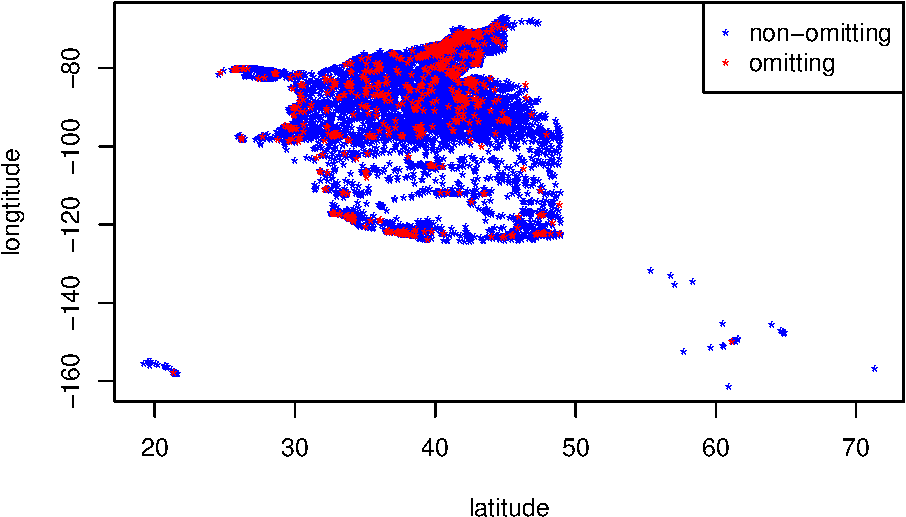
\includegraphics{./writeup_files/figure-latex/unnamed-chunk-2.pdf}

We can see from the graph that although there is a slight correlation
between omitting these questions and geographic location, the connection
is not conclusive.

\section{Relations between questions and geographic
location}\label{relations-between-questions-and-geographic-location}

We will first look at the relations between some of the questions and
location by inspecting the results of Hierarchical Clustering and
K-means Clustering

\begin{Shaded}
\begin{Highlighting}[]
\NormalTok{binary.data =}\StringTok{ }\KeywordTok{read.table}\NormalTok{(}\StringTok{"binary-ling-data.data"}\NormalTok{, }\DataTypeTok{header=}\NormalTok{T)}
\CommentTok{# since hclust has a running time much worse than kmeans, we use a sampled set here to explore}
\NormalTok{sampled =}\StringTok{ }\KeywordTok{sample}\NormalTok{(}\DataTypeTok{x=}\DecValTok{1}\NormalTok{:}\KeywordTok{nrow}\NormalTok{(binary.data), }\DataTypeTok{size=}\DecValTok{5966}\NormalTok{)}
\NormalTok{binary.data.sampled =}\StringTok{ }\NormalTok{binary.data[sampled,]}
\NormalTok{binary.vars =}\StringTok{ }\KeywordTok{grep}\NormalTok{(}\StringTok{"Q"}\NormalTok{, }\KeywordTok{names}\NormalTok{(binary.data), }\DataTypeTok{value=}\NormalTok{T)}
\NormalTok{selected.vars =}\StringTok{ }\NormalTok{binary.vars[}\DecValTok{65}\NormalTok{:}\DecValTok{107}\NormalTok{] }\CommentTok{# Q60-64}
\NormalTok{binary.dist =}\StringTok{ }\KeywordTok{dist}\NormalTok{(binary.data.sampled[, selected.vars])}
\NormalTok{tree =}\StringTok{ }\KeywordTok{hclust}\NormalTok{(binary.dist)}
\NormalTok{hclust.labels =}\StringTok{ }\KeywordTok{cutree}\NormalTok{(tree, }\DataTypeTok{h=}\DecValTok{3}\NormalTok{)}
\NormalTok{colors =}\StringTok{ }\KeywordTok{rainbow}\NormalTok{(}\KeywordTok{max}\NormalTok{(hclust.labels))}\CommentTok{# brewer.pal(name='Blues',n=max(hclust.labels))}
\KeywordTok{plot}\NormalTok{(binary.data.sampled[, }\StringTok{"lat"}\NormalTok{], binary.data.sampled[, }\StringTok{"long"}\NormalTok{], }\DataTypeTok{col=}\NormalTok{colors[hclust.labels], }\DataTypeTok{xlab=}\StringTok{"latitude"}\NormalTok{, }\DataTypeTok{ylab=}\StringTok{"longtitude"}\NormalTok{, }\DataTypeTok{pch=}\DecValTok{20}\NormalTok{, }\DataTypeTok{main=}\StringTok{"Clusters from Hierarchical Clustering"}\NormalTok{)}
\end{Highlighting}
\end{Shaded}

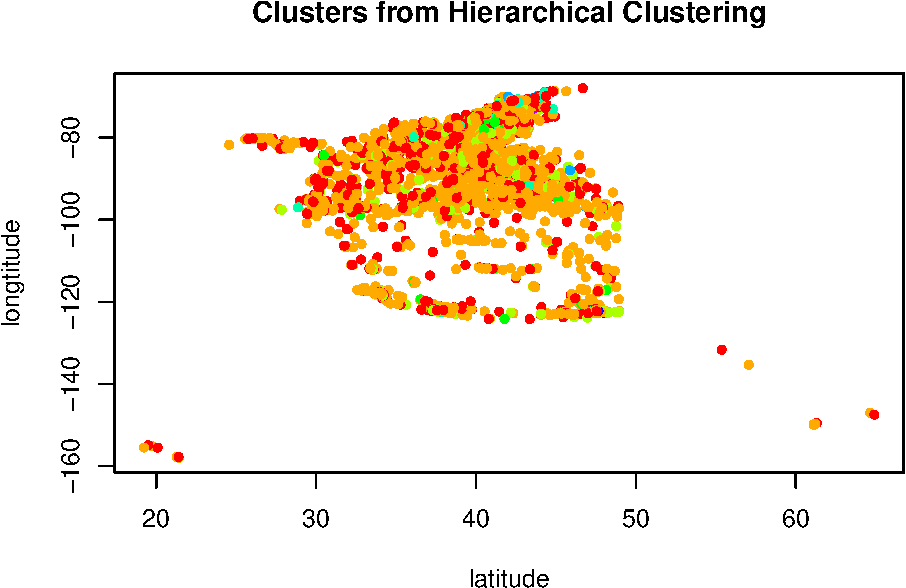
\includegraphics{./writeup_files/figure-latex/unnamed-chunk-31.pdf}

\begin{Shaded}
\begin{Highlighting}[]
\NormalTok{kmeans.labels =}\StringTok{ }\KeywordTok{kmeans}\NormalTok{(binary.data[, selected.vars], }\DataTypeTok{centers=}\KeywordTok{max}\NormalTok{(hclust.labels))$cluster}
\KeywordTok{plot}\NormalTok{(binary.data[, }\StringTok{"lat"}\NormalTok{], binary.data[, }\StringTok{"long"}\NormalTok{], }\DataTypeTok{col=}\NormalTok{colors[kmeans.labels], }\DataTypeTok{xlab=}\StringTok{"latitude"}\NormalTok{, }\DataTypeTok{ylab=}\StringTok{"longtitude"}\NormalTok{, }\DataTypeTok{pch=}\DecValTok{20}\NormalTok{, }\DataTypeTok{main=}\StringTok{"Clusters from K-means"}\NormalTok{)}
\end{Highlighting}
\end{Shaded}

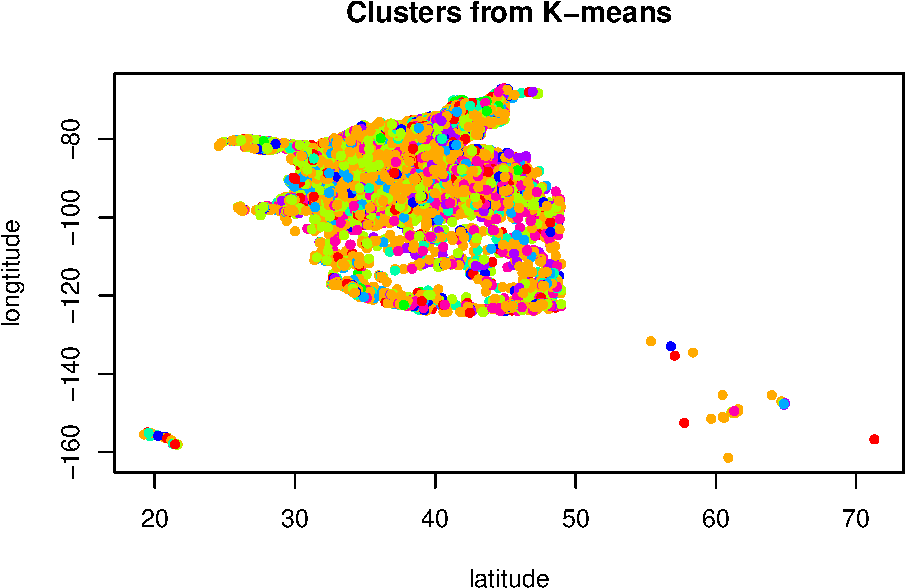
\includegraphics{./writeup_files/figure-latex/unnamed-chunk-32.pdf}

From both the results of K-means and Hierarchical Clustering, we can see
that there are dominant clusters that are distributed relatively
uniformly in terms of geographic-location. On the other hand, there
exist a certain number of smaller groups that exihbit stronger location
association. This phenomenon can be interpreted as certain dialects are
prevalent everywhere and hence do not indicate strong association with
specific areas. On the other hand, some dialects might be tied more
tightly to the locations that use the dialects.

Then we will investigate if we can use some questions to predict to
answers of others. If the answer is yes, then it would be safe to assume
that these questions do characterize different dialects. In particular,
we will try to use a subset of the binarified data to predict another
subset using multinomial logistic classification

\begin{Shaded}
\begin{Highlighting}[]
\NormalTok{train =}\StringTok{ }\KeywordTok{sample}\NormalTok{(}\DecValTok{1}\NormalTok{:}\KeywordTok{nrow}\NormalTok{(binary.data), }\DataTypeTok{size=}\DecValTok{5000}\NormalTok{)}
\NormalTok{test =}\StringTok{ }\KeywordTok{sample}\NormalTok{(}\KeywordTok{setdiff}\NormalTok{(}\DecValTok{1}\NormalTok{:}\KeywordTok{nrow}\NormalTok{(binary.data), train), }\DataTypeTok{size=}\DecValTok{5000}\NormalTok{)}

\NormalTok{predicted.vars =}\StringTok{ }\NormalTok{vars[}\DecValTok{1}\NormalTok{:}\DecValTok{11}\NormalTok{] }\CommentTok{# Q50-Q60}
\NormalTok{temp =}\StringTok{ }\KeywordTok{cbind}\NormalTok{(filtered.data[train, predicted.vars], binary.data[train, selected.vars])}
\KeywordTok{library}\NormalTok{(}\StringTok{"nnet"}\NormalTok{)}
\NormalTok{Mode <-}\StringTok{ }\NormalTok{function(x) \{}
  \NormalTok{ux <-}\StringTok{ }\KeywordTok{unique}\NormalTok{(x)}
  \NormalTok{ux[}\KeywordTok{which.max}\NormalTok{(}\KeywordTok{tabulate}\NormalTok{(}\KeywordTok{match}\NormalTok{(x, ux)))]}
\NormalTok{\}}
\NormalTok{for (q in predicted.vars) \{}
  \KeywordTok{sink}\NormalTok{(}\DataTypeTok{file=}\StringTok{"/dev/null"}\NormalTok{)}
  \NormalTok{multi =}\StringTok{ }\KeywordTok{multinom}\NormalTok{(}\KeywordTok{paste}\NormalTok{(q, }\StringTok{" ~ "}\NormalTok{, }\KeywordTok{paste}\NormalTok{(selected.vars, }\DataTypeTok{collapse=}\StringTok{"+"}\NormalTok{)), }\DataTypeTok{data =} \NormalTok{temp, }\DataTypeTok{maxit=}\DecValTok{500}\NormalTok{)}
  \KeywordTok{sink}\NormalTok{()}
  \NormalTok{predicted =}\StringTok{ }\KeywordTok{predict}\NormalTok{(multi, binary.data[test, selected.vars])}
  \NormalTok{actual =}\StringTok{ }\NormalTok{filtered.data[test, q]}
  \KeywordTok{print}\NormalTok{(}\KeywordTok{paste}\NormalTok{(}\StringTok{"Using answers from Q60-64 to classify answer of "}\NormalTok{, q))}
  \KeywordTok{print}\NormalTok{(}\StringTok{"Rate of naive classifier:"}\NormalTok{)}
  \KeywordTok{print}\NormalTok{(}\KeywordTok{sum}\NormalTok{(}\KeywordTok{Mode}\NormalTok{(actual) ==}\StringTok{ }\NormalTok{actual)/}\StringTok{ }\KeywordTok{length}\NormalTok{(test))}
  \KeywordTok{print}\NormalTok{(}\StringTok{"Rate of this classifier:"}\NormalTok{)}
  \KeywordTok{print}\NormalTok{(}\KeywordTok{sum}\NormalTok{(predicted ==}\StringTok{ }\NormalTok{actual) /}\StringTok{ }\KeywordTok{length}\NormalTok{(test))}
\NormalTok{\}}
\end{Highlighting}
\end{Shaded}

\begin{verbatim}
## [1] "Using answers from Q60-64 to classify answer of  Q050"
## [1] "Rate of naive classifier:"
## [1] 0.4124
## [1] "Rate of this classifier:"
## [1] 0.4328
## [1] "Using answers from Q60-64 to classify answer of  Q051"
## [1] "Rate of naive classifier:"
## [1] 0.6798
## [1] "Rate of this classifier:"
## [1] 0.6764
## [1] "Using answers from Q60-64 to classify answer of  Q052"
## [1] "Rate of naive classifier:"
## [1] 0.396
## [1] "Rate of this classifier:"
## [1] 0.396
## [1] "Using answers from Q60-64 to classify answer of  Q053"
## [1] "Rate of naive classifier:"
## [1] 0.8766
## [1] "Rate of this classifier:"
## [1] 0.8754
## [1] "Using answers from Q60-64 to classify answer of  Q054"
## [1] "Rate of naive classifier:"
## [1] 0.9146
## [1] "Rate of this classifier:"
## [1] 0.9146
## [1] "Using answers from Q60-64 to classify answer of  Q055"
## [1] "Rate of naive classifier:"
## [1] 0.8802
## [1] "Rate of this classifier:"
## [1] 0.8802
## [1] "Using answers from Q60-64 to classify answer of  Q056"
## [1] "Rate of naive classifier:"
## [1] 0.6162
## [1] "Rate of this classifier:"
## [1] 0.6272
## [1] "Using answers from Q60-64 to classify answer of  Q057"
## [1] "Rate of naive classifier:"
## [1] 0.69
## [1] "Rate of this classifier:"
## [1] 0.6892
## [1] "Using answers from Q60-64 to classify answer of  Q058"
## [1] "Rate of naive classifier:"
## [1] 0.5434
## [1] "Rate of this classifier:"
## [1] 0.5576
## [1] "Using answers from Q60-64 to classify answer of  Q059"
## [1] "Rate of naive classifier:"
## [1] 0.5006
## [1] "Rate of this classifier:"
## [1] 0.4966
## [1] "Using answers from Q60-64 to classify answer of  Q060"
## [1] "Rate of naive classifier:"
## [1] 0.6326
## [1] "Rate of this classifier:"
## [1] 1
\end{verbatim}

We will use the constant function $f(x) = Mode(X)$ as a baseline naive
classifier to compare the multinomial classifier's performance. The fact
that these naive classifiers can sometimes outperform naive classifiers
suggest a certain level of connection between some of these questions,
but it also revelas that there might not be associations between certain
pairs of questions.

\section{Dimensionality Reduction}\label{dimensionality-reduction}

Since it's hard to explore high-dimensional data, we will apply the
usual dimensionality reduction technique to aid our exploration. Notice
here it doesn't make sense to apply PCA to the raw responses data,
because the discrete values in each dimension (responses to questions)
do not admit proper interpretation in real number domain.

\begin{Shaded}
\begin{Highlighting}[]
\CommentTok{# again, we use a sampled set instead of the whole data set}
\NormalTok{pca =}\StringTok{ }\KeywordTok{prcomp}\NormalTok{(binary.data[, binary.vars])}
\CommentTok{# look at summary}
\CommentTok{# summary(pca)}
\NormalTok{## Importance of components:}
\NormalTok{##                           PC1    PC2    PC3    PC4    PC5    PC6    PC7}
\NormalTok{## Standard deviation     1.2191 1.1252 1.0225 0.8773 0.8460 0.8111 0.7855}
\NormalTok{## Proportion of Variance 0.0411 0.0350 0.0289 0.0213 0.0198 0.0182 0.0171}
\NormalTok{## Cumulative Proportion  0.0411 0.0762 0.1051 0.1265 0.1463 0.1645 0.1816}
\NormalTok{trans =}\StringTok{ }\KeywordTok{solve}\NormalTok{(pca$rotation)}
\KeywordTok{par}\NormalTok{(}\DataTypeTok{mfrow=}\KeywordTok{c}\NormalTok{(}\DecValTok{3}\NormalTok{,}\DecValTok{1}\NormalTok{))}
\KeywordTok{barplot}\NormalTok{(trans[}\StringTok{"PC1"}\NormalTok{, ], }\DataTypeTok{main=}\StringTok{"Contribution to First PC"}\NormalTok{)}
\KeywordTok{barplot}\NormalTok{(trans[}\StringTok{"PC2"}\NormalTok{, ], }\DataTypeTok{main=}\StringTok{"Contribution to Second PC"}\NormalTok{)}
\KeywordTok{barplot}\NormalTok{(trans[}\StringTok{"PC3"}\NormalTok{, ], }\DataTypeTok{main=}\StringTok{"Contribution to Third PC"}\NormalTok{)}
\end{Highlighting}
\end{Shaded}

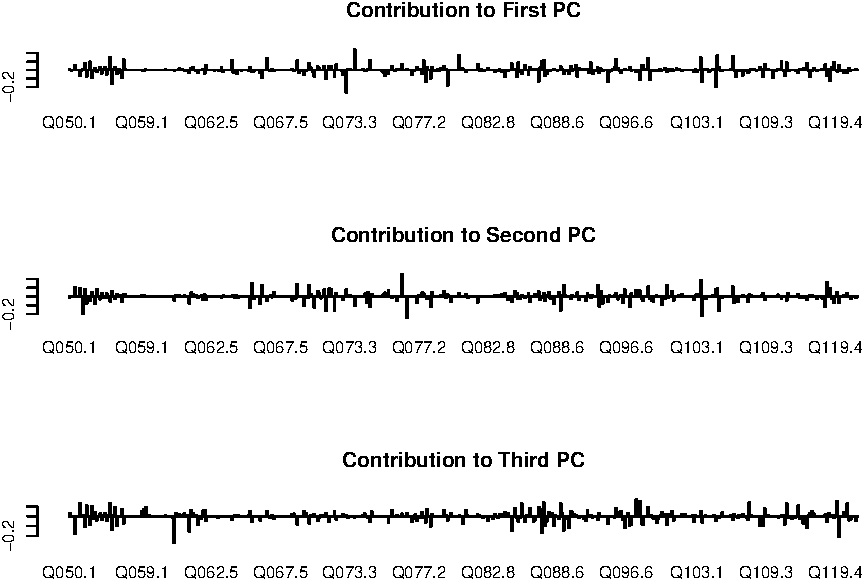
\includegraphics{./writeup_files/figure-latex/unnamed-chunk-51.pdf}

\begin{Shaded}
\begin{Highlighting}[]
\NormalTok{pca.scaled =}\StringTok{ }\KeywordTok{prcomp}\NormalTok{(binary.data[, binary.vars], }\DataTypeTok{scale.=}\NormalTok{T)}
\CommentTok{# look at summary}
\CommentTok{# summary(pca.scaled)}
\NormalTok{## Importance of components:}
\NormalTok{##                           PC1    PC2    PC3    PC4    PC5    PC6     PC7}
\NormalTok{## Standard deviation     3.0254 2.7574 2.5768 2.3815 2.2235 2.1634 2.08508}
\NormalTok{## Proportion of Variance 0.0196 0.0163 0.0142 0.0121 0.0106 0.0100 0.00929}
\NormalTok{## Cumulative Proportion  0.0196 0.0358 0.0500 0.0621 0.0727 0.0827 0.09197}
\NormalTok{trans =}\StringTok{ }\KeywordTok{solve}\NormalTok{(pca.scaled$rotation)}
\KeywordTok{par}\NormalTok{(}\DataTypeTok{mfrow=}\KeywordTok{c}\NormalTok{(}\DecValTok{3}\NormalTok{,}\DecValTok{1}\NormalTok{))}
\KeywordTok{barplot}\NormalTok{(trans[}\StringTok{"PC1"}\NormalTok{, ], }\DataTypeTok{main=}\StringTok{"Contribution to First PC"}\NormalTok{)}
\KeywordTok{barplot}\NormalTok{(trans[}\StringTok{"PC2"}\NormalTok{, ], }\DataTypeTok{main=}\StringTok{"Contribution to Second PC"}\NormalTok{)}
\KeywordTok{barplot}\NormalTok{(trans[}\StringTok{"PC3"}\NormalTok{, ], }\DataTypeTok{main=}\StringTok{"Contribution to Third PC"}\NormalTok{)}
\end{Highlighting}
\end{Shaded}

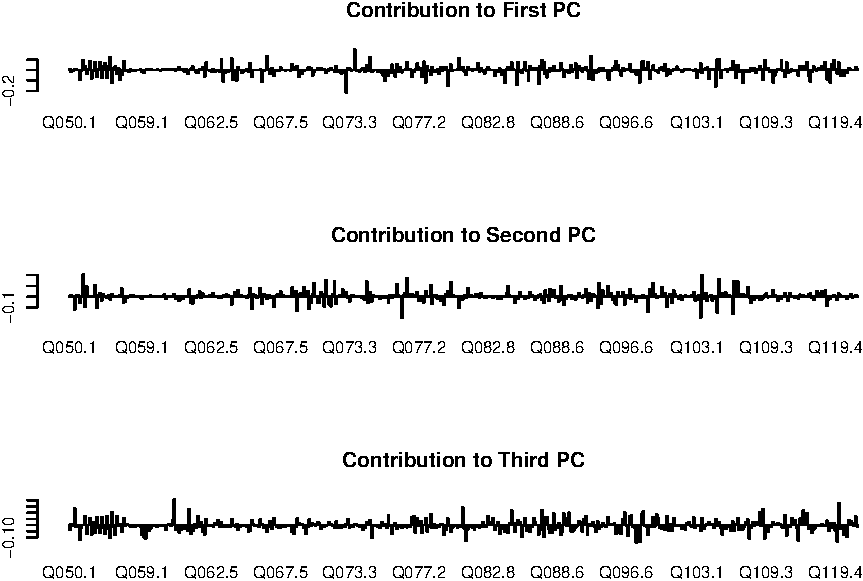
\includegraphics{./writeup_files/figure-latex/unnamed-chunk-52.pdf}

We can observe that scaling the variables has a considerable effect on
the results of PCA. This is expected since some of the dimensions
contain extremely sparse data which make the absolute variance of that
dimension smaller in comparison with others. Hence after scaling we can
see that more variables have significant roles in the important
principle components.

\begin{Shaded}
\begin{Highlighting}[]
\NormalTok{contrib =}\StringTok{ }\KeywordTok{apply}\NormalTok{(}\KeywordTok{abs}\NormalTok{(trans)[}\DecValTok{1}\NormalTok{:}\DecValTok{4}\NormalTok{, ], }\DataTypeTok{FUN=}\NormalTok{sum, }\DataTypeTok{MARGIN=}\KeywordTok{c}\NormalTok{(}\DecValTok{2}\NormalTok{))}
\NormalTok{ind =}\StringTok{ }\KeywordTok{which}\NormalTok{(contrib >=}\StringTok{ }\KeywordTok{quantile}\NormalTok{(contrib, }\DataTypeTok{probs=}\KeywordTok{c}\NormalTok{(}\FloatTok{0.99}\NormalTok{)))}
\NormalTok{significant.vars =}\StringTok{ }\NormalTok{binary.vars[ind]}
\end{Highlighting}
\end{Shaded}

We can see that Questions 50, 86, 99, 105 and 115 are given more weights
in principle components.

\section{Clustering with Reduced-Dimension
Data}\label{clustering-with-reduced-dimension-data}

By choosing first few principle components from PCA, we can presumably
preserve most intrinsic variation and get rid of noise. Hence it makes
sense to revisit the problem of clustering with the reduced data. Here
we will be using K-means to explore varying number of clusters.

\begin{Shaded}
\begin{Highlighting}[]
\NormalTok{reduced =}\StringTok{ }\NormalTok{pca.scaled$x[, }\DecValTok{1}\NormalTok{:}\DecValTok{217}\NormalTok{] }\CommentTok{# to account for 70% of the observed variance}
\KeywordTok{par}\NormalTok{(}\DataTypeTok{mfrow=}\KeywordTok{c}\NormalTok{(}\DecValTok{1}\NormalTok{,}\DecValTok{2}\NormalTok{))}
\KeywordTok{library}\NormalTok{(RColorBrewer)}
\NormalTok{for (k in }\DecValTok{3}\NormalTok{:}\DecValTok{7}\NormalTok{) \{}
  \NormalTok{colors =}\StringTok{ }\KeywordTok{brewer.pal}\NormalTok{(k,}\StringTok{"Set3"}\NormalTok{)}
  \NormalTok{clusters =}\StringTok{ }\KeywordTok{kmeans}\NormalTok{(binary.data[, binary.vars], }\DataTypeTok{centers=}\NormalTok{k)$cluster}
  \KeywordTok{plot}\NormalTok{(binary.data[, }\StringTok{"lat"}\NormalTok{], binary.data[, }\StringTok{"long"}\NormalTok{], }\DataTypeTok{col=}\NormalTok{colors[clusters], }\DataTypeTok{xlab=}\StringTok{"latitude"}\NormalTok{, }\DataTypeTok{ylab=}\StringTok{"longtitude"}\NormalTok{, }\DataTypeTok{pch=}\DecValTok{20}\NormalTok{, }\DataTypeTok{main=}\KeywordTok{paste}\NormalTok{(}\StringTok{"k="}\NormalTok{,k))}
  \NormalTok{reduced.clusters =}\StringTok{ }\KeywordTok{kmeans}\NormalTok{(reduced, }\DataTypeTok{centers=}\NormalTok{k)$cluster}
  \KeywordTok{plot}\NormalTok{(binary.data[, }\StringTok{"lat"}\NormalTok{], binary.data[, }\StringTok{"long"}\NormalTok{], }\DataTypeTok{col=}\NormalTok{colors[reduced.clusters], }\DataTypeTok{xlab=}\StringTok{"latitude"}\NormalTok{, }\DataTypeTok{ylab=}\StringTok{"longtitude"}\NormalTok{, }\DataTypeTok{pch=}\DecValTok{20}\NormalTok{, }\DataTypeTok{main=}\KeywordTok{paste}\NormalTok{(}\StringTok{"(Dimension-reduced) k="}\NormalTok{,k))}
\NormalTok{\}}
\end{Highlighting}
\end{Shaded}

\includegraphics{./writeup_files/figure-latex/unnamed-chunk-71.pdf}
\includegraphics{./writeup_files/figure-latex/unnamed-chunk-72.pdf}
\includegraphics{./writeup_files/figure-latex/unnamed-chunk-73.pdf}
\includegraphics{./writeup_files/figure-latex/unnamed-chunk-74.pdf}
\includegraphics{./writeup_files/figure-latex/unnamed-chunk-75.pdf}

We can see that clusters are relatively stable between the learnt from
raw data and that from reduced data, except that in some cases the
reduced data could yield results that merge some distinct clusters. On
the other hand, as the number of clusters increases, the separability in
terms of geo-location beomes weaker, which suggests that either these
are dialects that are mixed in terms of geo-location or that these
clusters that overlap significantly represent indeed geographically
separate dialects but the survey questions cannot discern the
differences between them.

In the end, we will investigate when we vary the number of principle
components used, how stable is the clustering

\begin{Shaded}
\begin{Highlighting}[]
\KeywordTok{par}\NormalTok{(}\DataTypeTok{mfrow=}\KeywordTok{c}\NormalTok{(}\DecValTok{2}\NormalTok{,}\DecValTok{3}\NormalTok{))}
\NormalTok{for (i in }\KeywordTok{c}\NormalTok{(}\DecValTok{5}\NormalTok{, }\DecValTok{50}\NormalTok{, }\DecValTok{100}\NormalTok{, }\DecValTok{200}\NormalTok{, }\DecValTok{300}\NormalTok{, }\DecValTok{400}\NormalTok{)) \{}
  \NormalTok{reduced =}\StringTok{ }\NormalTok{pca.scaled$x[, }\DecValTok{1}\NormalTok{:i]}\CommentTok{# to account for 70% of the observed variance}
  \NormalTok{k=}\DecValTok{5}
\KeywordTok{library}\NormalTok{(RColorBrewer)}
  \NormalTok{colors =}\StringTok{ }\KeywordTok{brewer.pal}\NormalTok{(k,}\StringTok{"Set3"}\NormalTok{)}
  \NormalTok{reduced.clusters =}\StringTok{ }\KeywordTok{kmeans}\NormalTok{(reduced, }\DataTypeTok{centers=}\NormalTok{k)$cluster}
  \KeywordTok{plot}\NormalTok{(binary.data[, }\StringTok{"lat"}\NormalTok{], binary.data[, }\StringTok{"long"}\NormalTok{], }\DataTypeTok{col=}\NormalTok{colors[reduced.clusters], }\DataTypeTok{xlab=}\StringTok{"latitude"}\NormalTok{, }\DataTypeTok{ylab=}\StringTok{"longtitude"}\NormalTok{, }\DataTypeTok{pch=}\DecValTok{20}\NormalTok{, }\DataTypeTok{main=}\KeywordTok{paste}\NormalTok{(}\StringTok{"k=5, PC="}\NormalTok{,i))}
\NormalTok{\}}
\end{Highlighting}
\end{Shaded}

\includegraphics{./writeup_files/figure-latex/unnamed-chunk-8.pdf}

From the above graph, we can see that albeit preserving general shape,
the clustering is not very stable as the number of principle components
used changes. It's also remarkable that using just $5$ components can
uncover almost as much structure as using many components.

\end{document}
